\section{Prototyping} %specifict prototyping
A prototype is an instantiation of a design concept meant for describing, refining, testing, and depicting the product.\cite{BUXTON2007139_prototyping}

When designing prototypes, the emphasis is not on the discovery of new knowledge and user needs, but to examine whether or not the proposed design constitutes a suitable hypothesis for the design of the product\cite{nielsen-norman-prototype-low-vs-high,BUXTON2007139_prototyping}.
That is, the design must allow for pleasurable interaction and suit user needs to a degree deemed adequate by both user and designer.

In general, two categories of prototypes exist: High Fidelity (hifi) and Low Fidelity (lofi).
Lofi prototypes are typically limited in their function and are used to emphasize concepts within the design, alternative design solutions, and model the general interaction with the artifact or system\cite{low-vs-high-fidelity-prototype}.
These prototypes are helpful when performing ideation\cite{nielsen-norman-ideation} or when establishing user capabilities in terms of interaction with the system \cite{usefullness-of-different-prototypes,low-vs-high-fidelity-prototype}.
Lofi prototypes should be used early in the design process to establish the overall direction for a product design. 
Therefore, the creation of these prototypes and the following evaluations using them should not be a time-consuming or expensive process. \cite{usefullness-of-different-prototypes,low-vs-high-fidelity-prototype} 
Lofi prototypes are not ideal when evaluating user interaction as they are used to present a design idea to the user, and thus are not interacted with by the user\cite{low-vs-high-fidelity-prototype}.

Unlike lofi prototypes, hifi prototypes provide near-complete functionality and interactivity with a design closely representing the final product.
They enable users to interact with buttons, icons, and input fields.
However, due to their detailed and interactive nature, constructing hifi prototypes is more time-consuming than creating lofi prototypes. 
This makes hifi prototypes more suitable for examining users' interactions with the designed artifact, than exploring new design ideas. \cite{nielsen-norman-prototype-low-vs-high,low-vs-high-fidelity-prototype}

Since the stakeholder has already suggested ideas for a user interface design based on existing systems and the use cases defined in Appendix \ref{appendix:user_stories}, we already have a direction for an initial product design. 
As we want to establish whether a system based on the user stories sufficiently solves the stakeholders' problems, we need to evaluate how users interact with a potential system.
For system evaluations a hifi prototype is more suitable than a lofi prototype \cite{low-vs-high-fidelity-prototype}.

\subsection{Developing prototypes}
When designing a product, multiple approaches can be taken.  
UCD aims to increase effectiveness, accessibility, and sustainability, as well as increase the pleasure the user experiences when using the system\cite{user-centred-design}. 
An alternative to UCD is LeanUX \cite{Lean_UX}.
Lean UX is also a user centered approach for UX development that is often used in start-ups.
The approach focusses on creating minimal viable products(MVPs) that can be iteratively released and tested with representative users. 
In this project, the stakeholder has suggested that we based our design on existing solutions.
Therefore, we endeavor towards a design strategy where we base the design on the current state-of-the-art systems for meeting-management and preferences of the stakeholders in the form of the user stories in Appendix \ref{appendix:user_stories}.
This makes UCD a prefered design strategy, as it focuses on increasing the effectiveness on the system.
In the context of the system we will develop, effectiveness will consider how well user stories are supported, and how suitable the system is for solving the problematic situation described in Section \ref{sec:understanding_the_problem}.

To develop the prototypes, the sketching tool Figma is used \cite{Figma}.
Figma can be used to design both high- and low-fidelity prototypes. 
It enables the designer to easily create a lofi prototype, and then later refine it such that users can interact with it.
Figma also contains a rich set of user interface components that can be used and modified when creating prototypes.
When a user interacts with a hifi prototype, by, for instance, clicking a UI element, the designer can enable a transition to a different view, thus simulating system UI behavior.
Based on the initial interviews described in Section \ref{sec:understanding_the_problem}, the prototypes must be suitable for use on a simple monitor, such as a tablet.

During this project, both a lofi and hifi prototype has been developed.
Each prototype shows a UI highlighting two situations for meeting rooms. 
The situations depict different states of a meeting room (occupied or available) which allows us to explore how users want to interact with the system in these different situations. 


\begin{figure}
    \centering
    \begin{subfigure}[b]{0.49\textwidth}
        \centering
        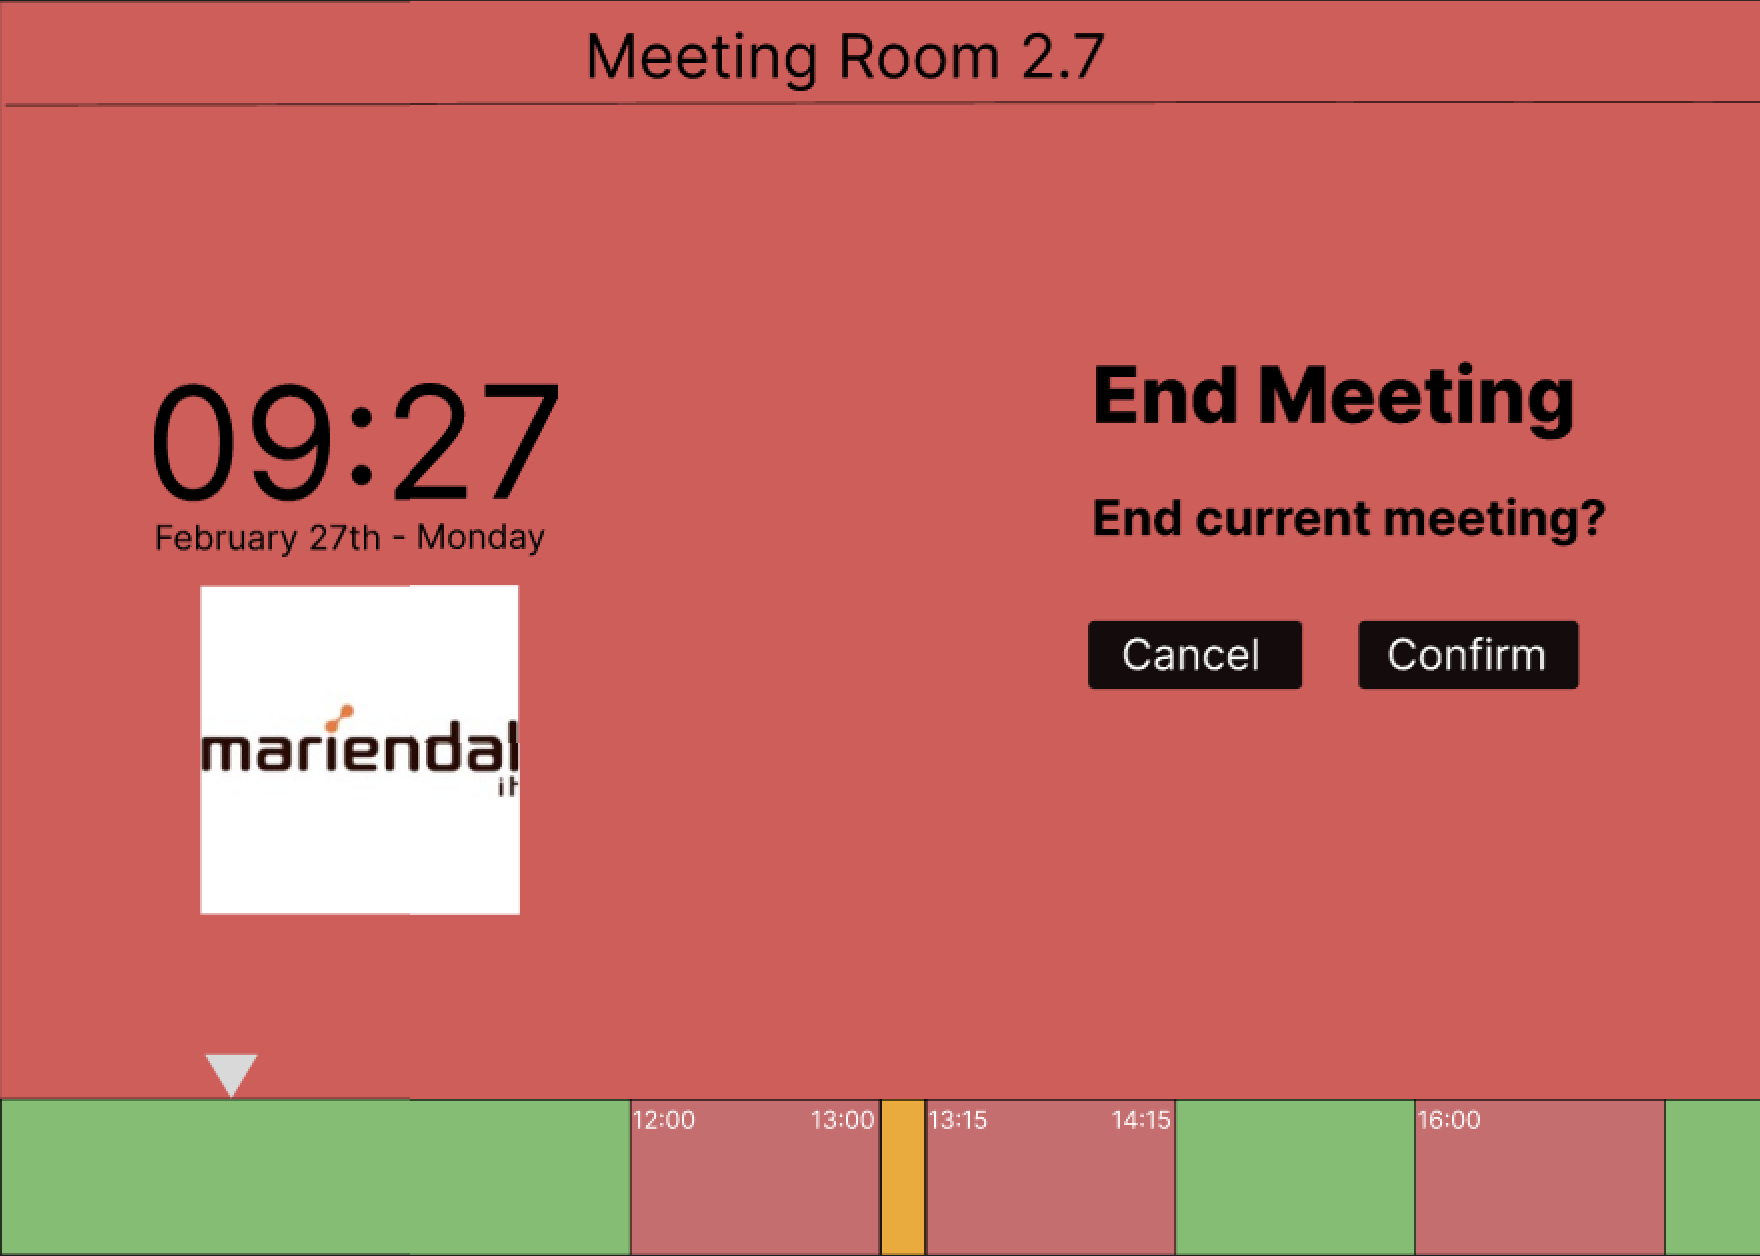
\includegraphics[width=\textwidth]{images/lofi_end.png}
        \caption{Tablet view for when a meeting room is occupied.}
        \label{fig:lofi_prototype:a}
    \end{subfigure}
    \begin{subfigure}[b]{0.49\textwidth}
        \centering
        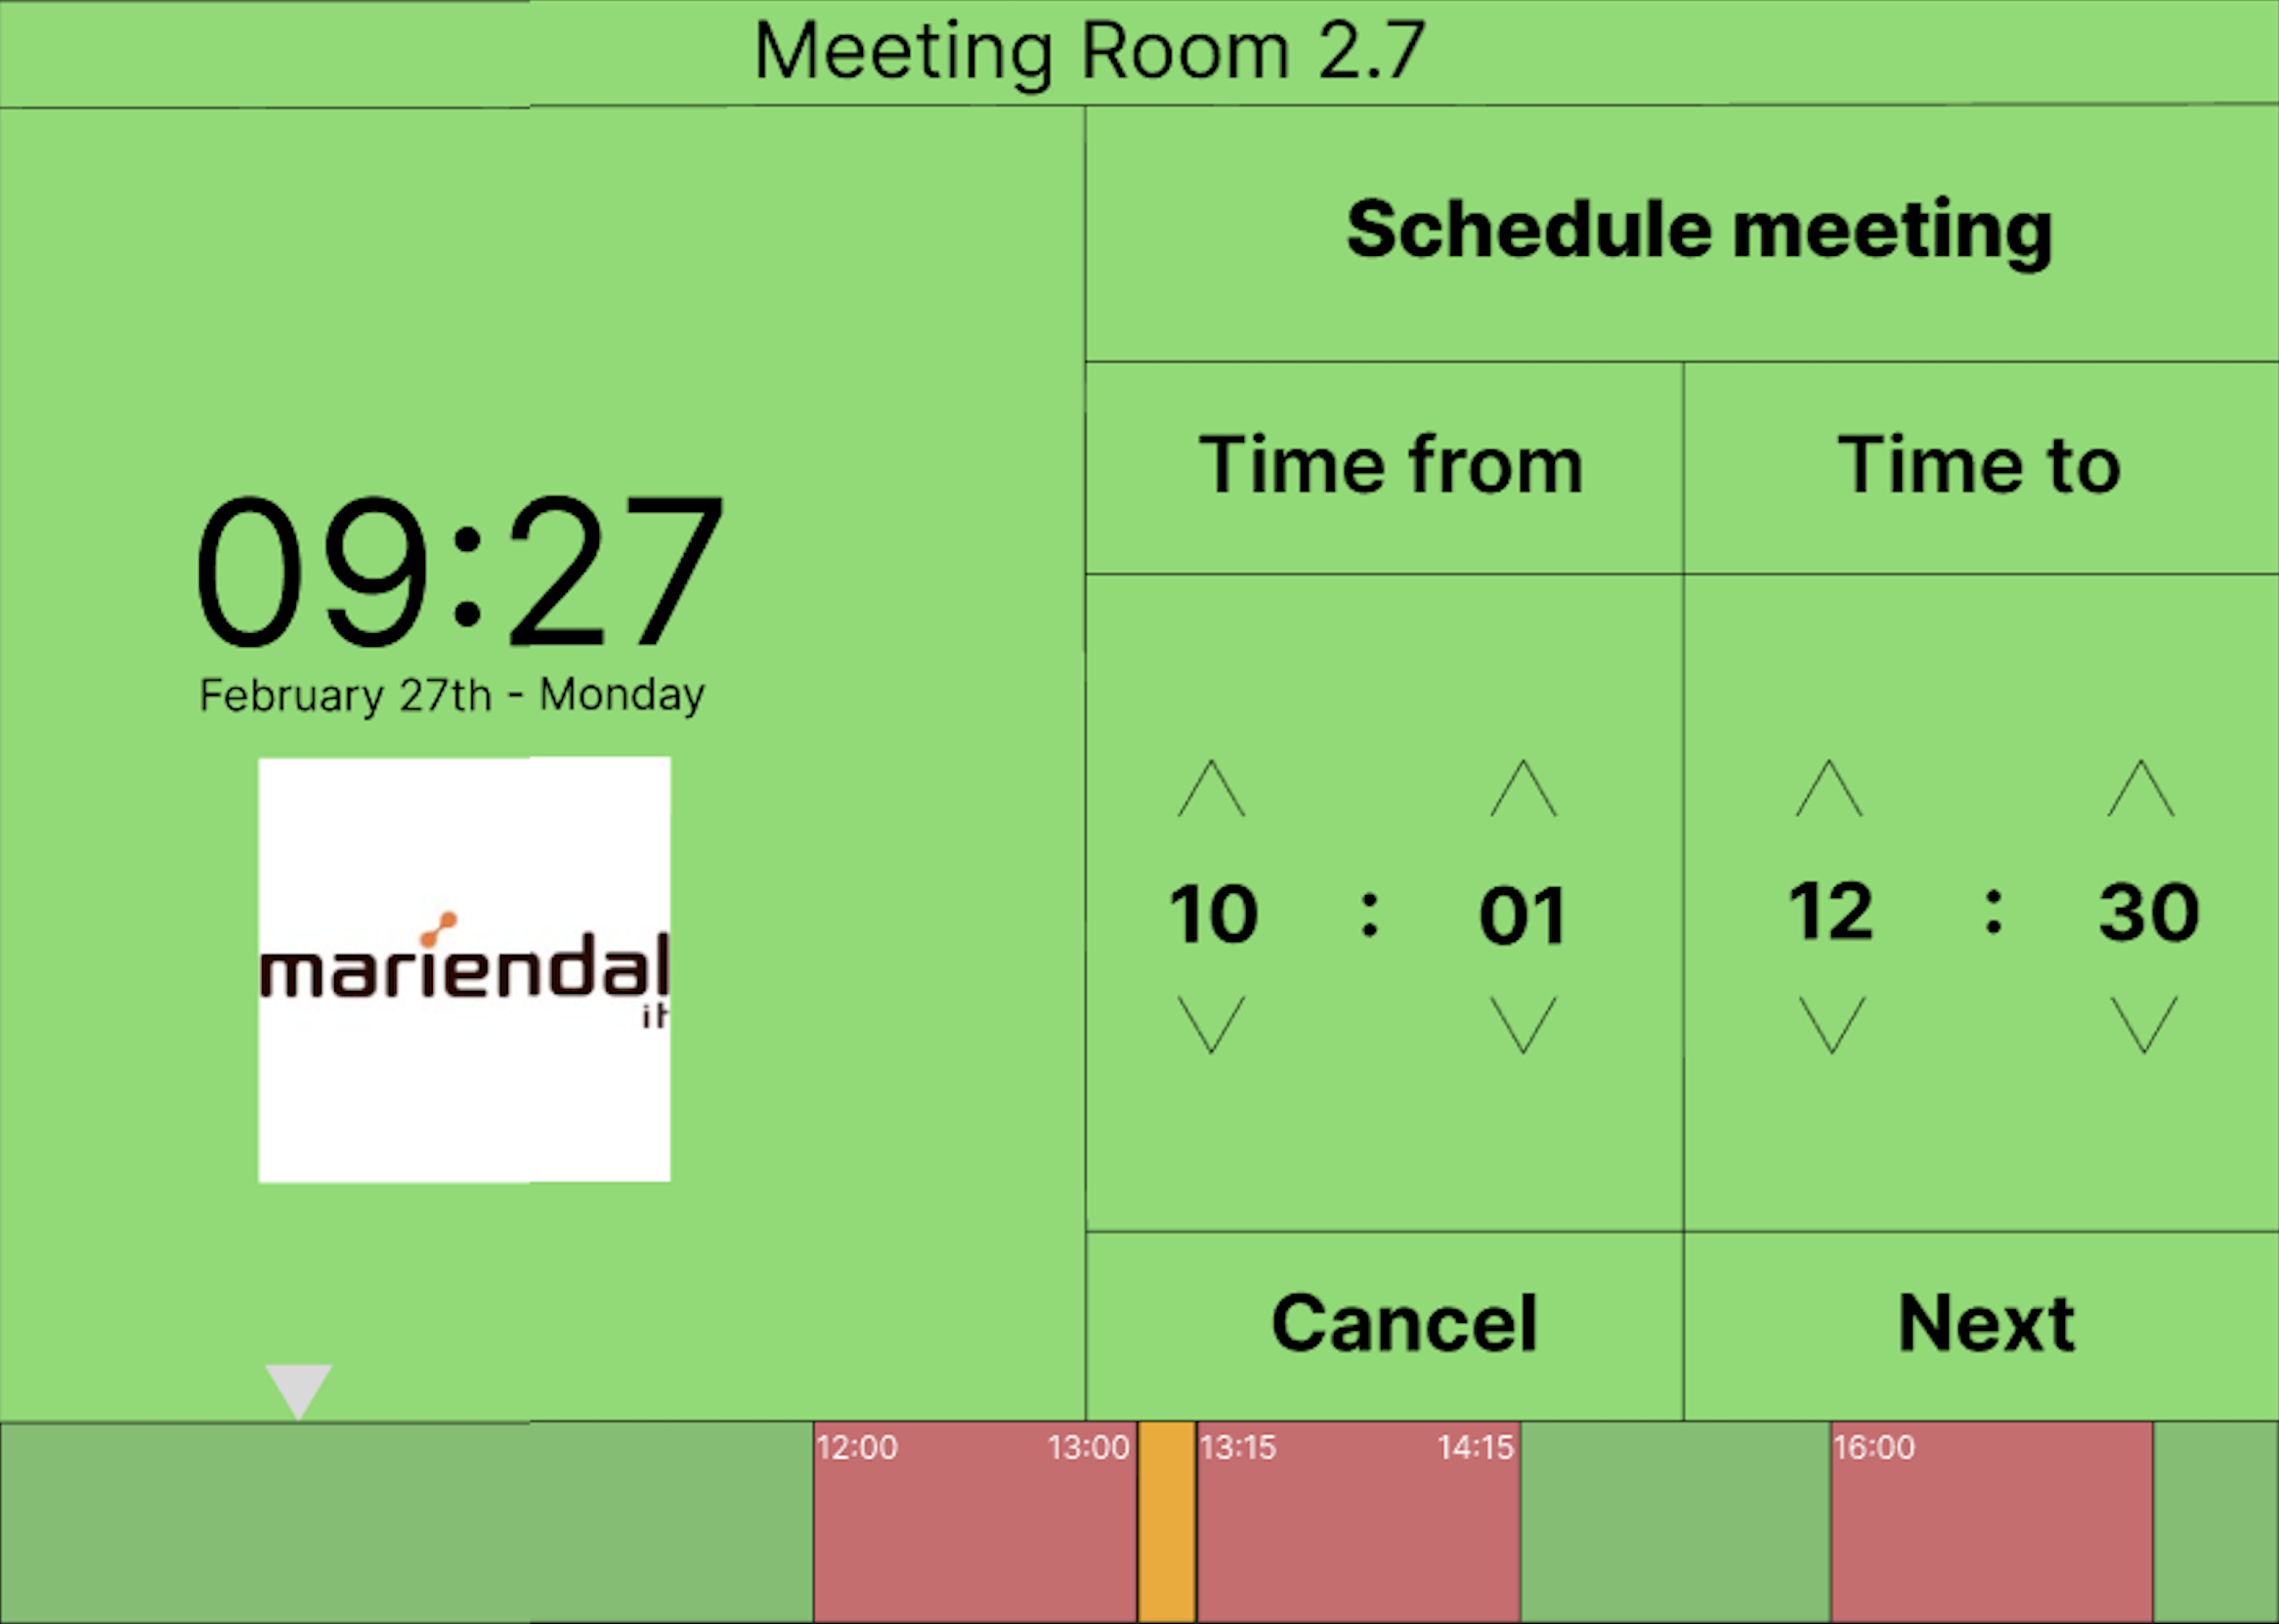
\includegraphics[width=\textwidth]{images/lofi_schedule.png}
        \caption{Tablet view for when a meeting room is available}
        \label{fig:lofi_prototype:b}
    \end{subfigure}
    \caption{Two views of the low fidelity prototype, each enabling different actions based on the state of the meeting room.}
    \label{fig:lofi_prototype}
\end{figure}

The development of a lofi prototype has been used as an internal exercise, independent from stakeholders, to explore initial design ideas based on existing systems.
Figure \ref{fig:lofi_prototype} depicts two views from the prototype, each based on the current state of the meeting room.
Depending on the state of the room, the background color as well as the actions available for the user changes.
Figure \ref{fig:lofi_prototype:a} depicts a view shown when a meeting is occupied.
Here, the main action available is to end the current meeting.
Figure \ref{fig:lofi_prototype:b} depicts a view shown when a meeting room is available.
From this view, the main action is to book the meeting room.

Based on this prototype, multiple ideas for a hifi prototype were conceived.
These ideas were filtered, refined, and turned into a single hifi prototype.
Figure \ref{fig:hifi_prototype_interaction} depicts the view for the same situations shown in Figure \ref{fig:lofi_prototype:a} where a room is occupied.
The hifi prototype enables user interaction with all elements that would be interactive in a final design.
Each user interaction with an interactive element changes what is shown on the prototype. 
This is shown in Figure \ref{fig:hifi_prototype_interaction}. 
All views for the hifi prototype can be found in Appendix \ref{appendix:hifi_prototype}.

\begin{figure}
    \centering
    \begin{subfigure}[b]{0.49\textwidth}
        \centering
        \includegraphics[width=\textwidth]{images/occupied_main_hifi.pdf}
        \caption{Tablet view depicting the design for when a meeting room is occupied.}
        \label{fig:hifi_prototype:a}
    \end{subfigure}
    \begin{subfigure}[b]{0.49\textwidth}
        \centering
        \includegraphics[width=\textwidth]{images/occupied_end_meeting.pdf}
        \caption{Tablet view asking for confirmation when ending a meeting.}
        \label{fig:hifi_prototype:b}
    \end{subfigure}
    \caption{Two views of the high fidelity prototype. When the user interacts with the 'End meeting' botton in Figure \ref{fig:hifi_prototype:a} the view is changed to what is depicted in Figure \ref{fig:hifi_prototype:b}}
    \label{fig:hifi_prototype_interaction}
\end{figure}
